% CHAPTER 1
\chapter{Introduction}
\section{Overview}
Biometric security is a mechanism which is used to authenticate and ....
\section{Motivation and Objectives} 
..To detect these fingerprint spoofing .... etc.

\section{Report Organization}
This section gives the organization of the report work. Overall, this report work gives a clear and thorough study about the existing study of the proposed system and gives a description about the implementation details. The second chapter gives a detailed description about the literature survey. Third chapter gives a brief idea about the implementation details including hardware and software requirements, outline of the proposed methodology. Fourth chapter depicts the Results and Discussions and fifth Chapter gives the Conclusion and Future Work. The Appendix shows the Screen Shots and Sample Code of the proposed systems.
\chapter{Literature Survey}
\section{Discussion of earlier/older works}
The Fingerprint Recognition System has ubiquitous deployment in many day-to-day applications, such as financial transactions, international border security, unlocking a smart phone\cite{1}

\paragraph{\textbf{Introduction}}
The Fingerprint Recognition System has ubiquitous deployment in many day-to-day applications, such 
as financial transactions,\cite{4} international border security, unlocking a smart phone, etc.
\section{Create appropriate subheadings}
This paper proposes a method to obtain the discriminant features for fingerprints whether they are real or spoofed, by performing feature level extractions \cite{10}. The fingerprint image is preprocessed using five preprocessing operations. The preprocessing operations were selected which have the lowest validation errors.
 \begin{enumerate}
\item Image reduction with different ratios Images are reduced using ``Bilinear Interpolation". They are used to verify the effect of resolution on the classifier performance. 
 \item Region Of Interest (ROI) Many fingerprints from some datasets are not centered; background represents large part of image. To input the classification system the largest area that comprises foreground fingerprints, a simple ROI method is used. 
\end{enumerate}
They are used to verify the effect of resolution on the classifier performance.They are used to verify the effect of resolution on the classifier performance. They are used to verify the effect of resolution on the classifier performance. They are used to verify the effect of resolution on the classifier performance. They are used to verify the effect of resolution on the classifier performance.
\chapter{Proposed Methodology}
\section{Add required subtopics as per paper}
\subsection{Xyz}
Research Methods: Description of the methods and techniques used in the paper.\\
Data Collection: How data was gathered, if applicable.\\
Experimental Setup: Details of any experiments or simulations conducted.\\
Key Topics: Detailed discussion of the main topics covered in the paper.\\
Figures/Tables: Include and describe any figures, tables, or charts used in the paper for better understanding.


\paragraph{}MATLAB supports graphical user interface (GUI) features for developing applications. For graphically designing these GUIs, MATLAB includes a GUIDE (GUI development environment) which also..

\section{Xy Z}
\subsection{Xy Z} 
From these, only Digital-Persona was selected for the training and testing process in order to reduce the time required for processing. It consists of 1000 live images in both training as well as testing sets whereas fake images are obtained from four materials ie. Ecoflex 

\subsection{Xy Z}
\textbf{Wave Atom Transformation for Image Enhancement}
The fingerprint images obtained from the LivDet 2015 datasets may contain some noise....
 and assigned it with two values 1 and 2. If the predicted value is 1, then it is considered as LIVE else it is FAKE.
    
\chapter{Results and Discussions}
This section gives as a detailed analysis of the proposed approach. 
Findings: Summary of the key findings or results presented.\\
Summary of Key Findings: Major takeaways from the seminar.\\
Analysis: Critical analysis of the information presented, including insights and implications.
\\We evaluated the performance on three scenarios to compare which one provides better performance.
\paragraph{ Evaluation of CNN with feature vector as input}
In this setting, the fingerprint images in the dataset are firstly enhanced using Wave Atom Transformation method in order to remove the unwanted noise from the image pixels..... It took only 00:00:20 hrs at the time of testing whereas other two methods took more time. Figure \ref{fig4.1} shows the gradient value obtained in each case. The performance Table \ref{tab:22}  depicts that Ecoflex 00-50 
\begin{figure}[h]
\centering
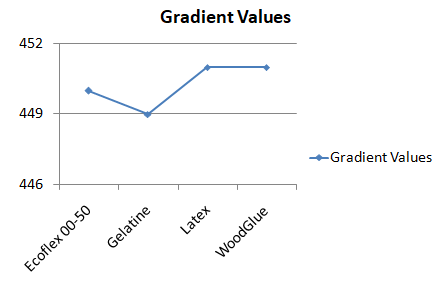
\includegraphics[scale=0.9]{Gradient.PNG}   
\caption{Graphical representation of gradient value obtained by each materials in the (ii) scenario}
\label{fig4.1}
\end{figure}

\begin{table}[h] 
\caption {Correct Rate and Error Rate obtained for CNN with feature vector as input} 
\label{tab:22} 
\center
\begin{tabular}{|c|c|c|}
\hline 
Materials Used (Live and Fake) & CR & ER\\ 
\hline 
Ecoflex 00-50 & 0.788 & 0.211 \\ 
\hline 
Gelatine & 0.808 & 0.192 \\ 
\hline 
Latex & 0.802 & 0.198 \\ 
\hline 
WoodGlue & 0.808 & 0.191 \\ 
\hline 
\end{tabular}
\end{table}

\chapter{Conclusion and Future Work}
The main limitation of many of the existing anti-spoof methods is the poor quality of the datasets obtained. The spoofing materials of poor image quality decreases the overall performance of the system. So we need either a best hardware for image acquisition or a good image processing method to obtain better results , but most of the hardware are expensive. 
\paragraph{}Here we proposed a method .....
The proposed WAT enhanced method yields an average accuracy of 85.8\%. The WAT enhanced image with minutiae features extracted, achieved an average accuracy of 79.8\%. We also computed the performance of CNN without any enhancement on image as input and obtained an average accuracy of 91.6\%.


